\section{Morris-Lecar}
The Morris-Lecar system is a concrete illustration of the exact stochastic simulation algorithms.
It was developed as a model for oscillation observed in barnacle muscle fibres.
The deterministic equations constitute a planar model for the evolution of the membrane potential $v(t)$ and the fraction of potassium gates $n\in[0,1]$ that are in the open state.
In addition to this there is a depolarizing current gated by a rapidly equilibrating variable $m$, the calcium conductance which is treated now as a fast, deterministic variable as in the standard fast/slow decomposition or the planar Morris-Lecar model.
The mean field equation for this model are:

\begin{align*}
	\frac{dv}{dt} = f(v, n) =& \frac{1}{C}(I_{app}-g_{Ca}m_{\infty}(v)(v-v_{Ca})+\\
													 &-g_L(v-v_L)-g_Kn(v-v_K))
\end{align*}

$$\frac{dn}{dt} = g(v, n) = \alpha(v)(1-n)-\beta(v)n = \frac{n_{\infty}(v)-n}{\tau(v)}$$

The kinetics of the potassium channel can be specified by the instantaneous time constant $\tau$, the asymptotic target $n_{\infty}$ or by the per capita transition rates $\alpha$ and $\beta$.
Moreover:

$$m_{\infty} = \frac{1}{2}\biggl(1+\tanh\biggl(\frac{v-v_a}{v_b}\biggr)\biggr)$$

$$\alpha(v) = \frac{\phi\cosh\bigl(\frac{\epsilon}{2}\bigr)}{1+e^{2\epsilon}}$$

$$\beta(v) = \frac{\phi\cosh\bigl(\frac{\epsilon}{2}\bigr)}{1+e^{-2\epsilon}}$$

$$n_\infty(v) = \frac{\alpha(v)}{\alpha(v)+\beta(v)} = \frac{1+\tanh\epsilon}{2}$$

$$\tau(v) = \frac{1}{\alpha(v)+\beta(v)} = \frac{1}{\phi\cosh\frac{\epsilon}{2}}$$

Where $\epsilon = \frac{v-v_c}{v_d}$ and the parameter will have values:

\begin{multicols}{3}
	\begin{itemize}
		\item $v_K = -84$.
		\item $v_L = -60$.
		\item $v_{Ca} = 120$.
		\item $I_{app} = 100$.
		\item $g_K = 8$.
		\item $g_L = 2$.
		\item $C = 20$.
		\item $v_a = -1.2$.
		\item $v_b = 18$.
		\item $v_c = 2$.
		\item $v_d = 30$.
		\item $\phi = 0.04$.
		\item $g_{Ca} = 4.4$.
	\end{itemize}
\end{multicols}

For which the deterministic system has a stable limit cycle.
For smaller values of the applied currents the system has a stable fixed point that loses stability through a subcritical Hopf bifurcation as $I_{app}$ increases.

	\subsection{Deterministic model}
	Before applying the two representation presented we implemented the Morris Lecar as a fully deterministic system abstracting from the single channel processes and using the asymptotic value $m_\infty$.
	We simulated it in Matlab using the variable order method \emph{ode15s} \cite{ode15s}.
	The behaviour of the model can be seen in figure \ref{fig:morris-lecar}.

	\begin{figure}
		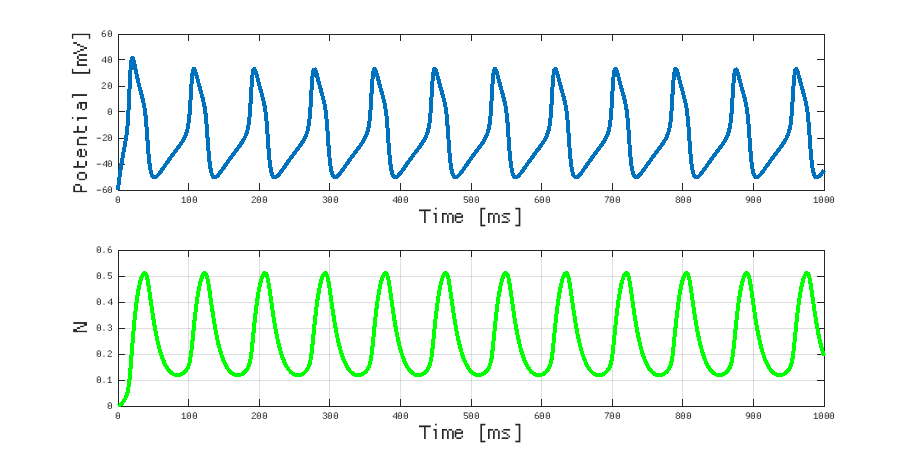
\includegraphics[width=\textwidth]{Figures/morris-lecar}
		\caption{Implementation of the fully deterministic Morris Lecar model. \textbf{TOP} Membrane potential. \textbf{Bottom} Fraction of open potassium channel.}
		\label{fig:morris-lecar}
	\end{figure}

	\subsection{Stochastic model}
	A finite number of potassium channels $N_{tot}$ is introduced and the number of open channels are treated as a discrete random process.
	Each potassium channel switches between the closed or open state independently of the other with voltage-dependent per capita transition rates $\alpha$ and $\beta$.
	The entire population conductance ranges from $0$ to $g_K^o = \frac{g_K}{N_{tot}}$.
	In this simulation $N_{tot} = 40$.
	The random variables will be the voltage and the number of open potassium channel.
	In the random time change representation the opening and closing of the potassium channels are driven by two independent unit rate Poisson processes $Y_{open}(t)$ and $Y_{close}(t)$.
	The evolutions  of $V$ and $N$ are linked.
	Whenever $N=n$, the evolution of $V$ obeys a deterministic differential equation:

	$$\frac{dV}{dt}\biggr\vert_{N=n} = f(V, n)$$

	$N$ evolves as a jump process: $N(t)$ is a piece-wise constant, with transitions occurring with intensities dependent on $V$.
	Whenever $V = v$:

	$$N\rightarrow N + 1\text{ net rate } \alpha(v)(N_{tot}-N)$$

	$$N\rightarrow N - 1\text{ net rate } \beta(v)N$$

	Now representing the state space for $N$ graphically:

	\begin{align*}
		0\xleftrightharpoons[\beta]{\alpha N_{tot}} 1 \xleftrightharpoons[2\beta]{\alpha(N_{tot}-1)}2\xleftrightharpoons[3\beta]{\alpha(N_{tot}-2)} \dots \xleftrightharpoons[k\beta]{\alpha(N_{tot}-k+1)}k&\\
		\scriptstyle{\alpha(N_{tot}-k)}\downharpoonleft\upharpoonright&\scriptstyle{(k+1)\beta}\\
		N_{tot}\xleftrightharpoons[N_{tot}\beta]{\alpha}(N_{tot}-1)\xleftrightharpoons[\beta(N_{tot}-1)]{2\alpha}\dots\xleftrightharpoons[(k+2)\beta]{\alpha(N_{tot}-k-1)}(k+1)&
	\end{align*}

The nodes represent possible states for process $N$ and the transition intensities located above and below the arrows.
Adopting the random time change representation the stochastic Morris-Lecar system is written as:

\begin{align*}
	\frac{dV}{dt} =& f(V(t), N(t)) = \\
								=& \frac{1}{C}(I_{app}-g_{Ca}m_\infty(V(t))(V(t)-V_{Ca})-g_L(V-V_L) +\\
								 &\qquad - g_K^oN(t)(V(t)-V_K))
\end{align*}

\begin{align*}
	N(t) = N(0) -&Y_{close}\biggl(\int_0^t\beta(V(s))N(s)ds\biggr) + \\
							 &Y_{open}\biggl(\int_0^t\alpha(V(s))(N_{tot}-N(s))ds\biggr)
\end{align*}

		\subsubsection{Random time change representation}
		We simulated the stochastic Morris Lecar model considering only the Potassium channel through the random time change representation for $4000$ seconds.
		The relationship within voltage and the number of open channel can be seen in figure \ref{fig:ml-rtc}.

		\begin{figure}
			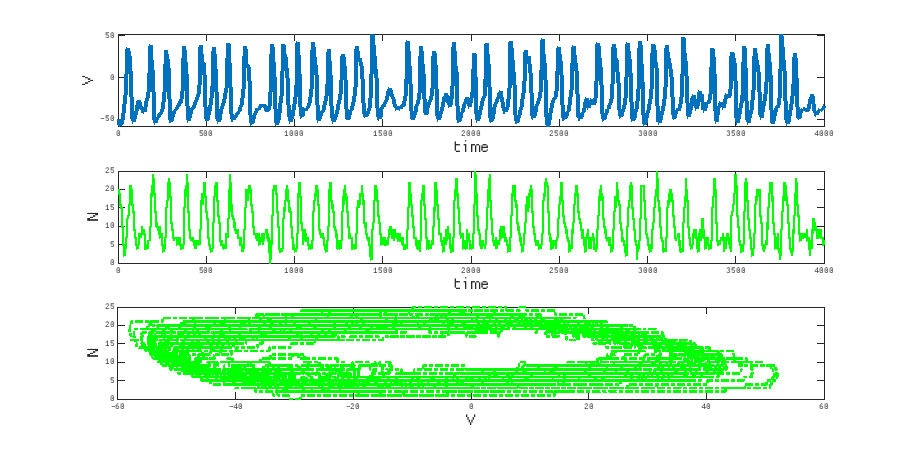
\includegraphics[width=\textwidth]{Figures/ml-rtc}
			\caption{The Morris Lecar stochastic model with only potassium channels. From top to bottom: \textbf{1} The membrane voltage. \textbf{2} The number of open potassium channel over time. \textbf{3} The number of open potassium channels over voltage.}
			\label{fig:ml-rtc}
		\end{figure}

		\subsubsection{Gillespie's representation}
		We simulated the stochastic Morris Lecar model considering only the Potassium channel through Gillespie's representation for $4000$ seconds.
		The relationship within voltage and the number of open channel can be seen in figure \ref{fig:ml-gill}.

		\begin{figure}
			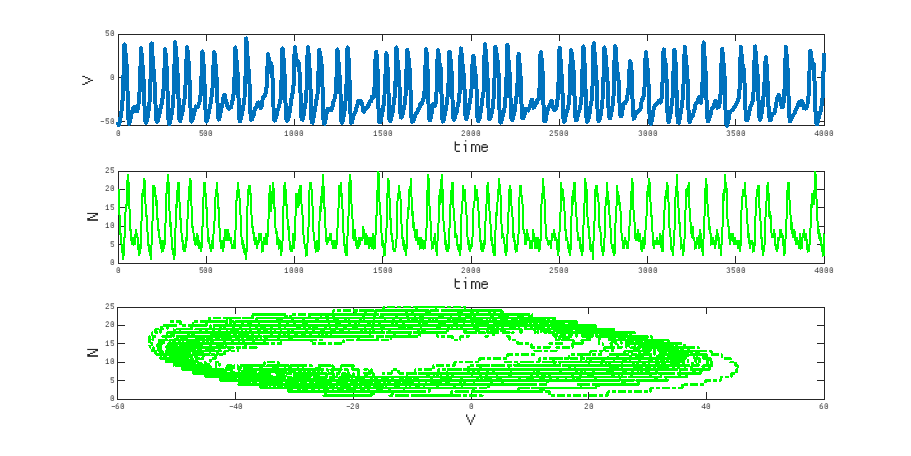
\includegraphics[width=\textwidth]{Figures/ml-gill}
			\caption{The Morris Lecar stochastic model with only potassium channels. From top to bottom: \textbf{1} The membrane voltage. \textbf{2} The number of open potassium channel over time. \textbf{3} The number of open potassium channels over voltage.}
			\label{fig:ml-gill}
		\end{figure}
